

\sujet{Mathematical geometry}

\noindent
{\bf Duration: 1h30 / 20 points}


\begin{note}
All documents allowed, NO internet connection (except for ecampus documents and language/function definitions). Please add comments and provide a code that can be executed without requiring any parameter.

It is highly recommended to reuse the codes made in the tutorials.
\end{note}

\section{Strauss point process (10 points)}

\subsection{Warm-up}

%\paragraph{0.} Code a function \texttt{Poisson\_Process(lambda,x\_size,y\_size)} that generates a Poisson point process of intensity $\lambda$ in a window of size $x\_size\times y\_size$.

Let $X$ be a set of points in two dimensions.

\begin{qbox}
Code a function \texttt{Count\_Pairs(X,R)} that counts the number of pairs of points in a set $X$ located at a distance less than $R$ (constant numerical value).
\end{qbox}

\subsection{Strauss point process}

We want to implement a function that returns a Strauss-like point process. A Strauss process is based on iterations upon a constrained\footnote{A constrained Poisson process has a fixed number of points which doesn't follow on a Poisson law anymore.} Poisson process in a window of size $[0;1]\times[0;1]$, where $X_0$ will denote the initial set of points. At each iteration, one of the points is slightly moved (e.g. according to a normal distribution of low variance, make a choice). We then consider the quantity $\alpha$ defined as follows:

\begin{enumerate}
\item[•] If the point leaves the observation window, it returns to its initial position, i.e. $\alpha=0$.
\item[•] If \texttt{Count\_Pairs(X$_{n+1}$,R)} is less than \texttt{Count\_Pairs(X$_{n}$,R)}, with $X_n$ the set of points at the iteration $n$ and $R$ a parameter of the process, then $\alpha=1$.
\item[•] Else $\alpha =\gamma^{\left(\texttt{Count\_Pairs}(X_{n+1},R)-\texttt{Count\_Pairs}(X_{n},R)\right)}$, with $\gamma$ a parameter of the process.
\item[•] Finally, a number $\beta$ is drawn randomly between 0 and 1. If $\beta<\alpha$, then the point set is updated with the shifted element. Otherwise, the original set is retained.
\end{enumerate}

\begin{qbox}

\begin{enumerate}
\item 
Code a function \texttt{Strauss(n,gamma,R,N)} that generates a Strauss point process of $n$ points and with parameters $\gamma\in[0;1]$, $R>0$ and $N$ the number of iterations.

\item Test your \texttt{Strauss(n,gamma,R,N)} function with $n=100$, $\gamma = 0.1$, $R=0.2$ and $N\geq 1000$ (example shown in Fig.\ref{subfig:agreg}).
\item Test your \texttt{Strauss(n,gamma,R,N)} function with $n=100$, $\gamma = 0.1$, $R=0.05$ and $N\geq 1000$ (example shown in Fig.\ref{subfig:regular}).
\item What happens if $\gamma = 1$? (example shown in Fig.\ref{subfig:poisson})
\end{enumerate}

\end{qbox}

\begin{figure}[htbp]
\subfloat[]{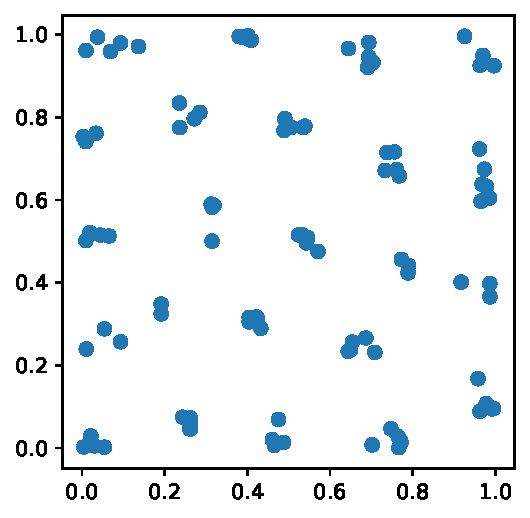
\includegraphics[width=.3\textwidth]{agreg.pdf}\label{subfig:agreg}}
\hfill
\subfloat[]{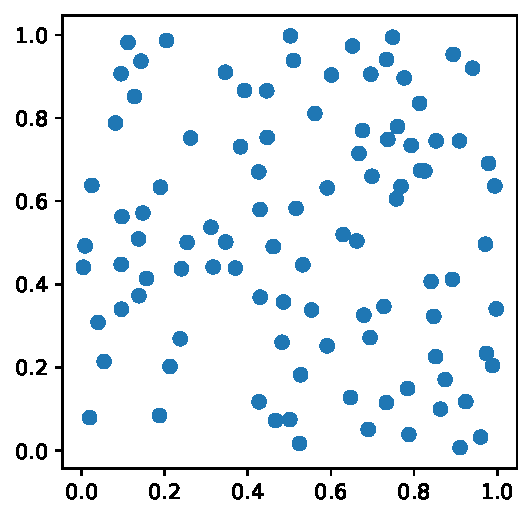
\includegraphics[width=.3\textwidth]{regular.pdf}\label{subfig:regular}}
\hfill
\subfloat[]{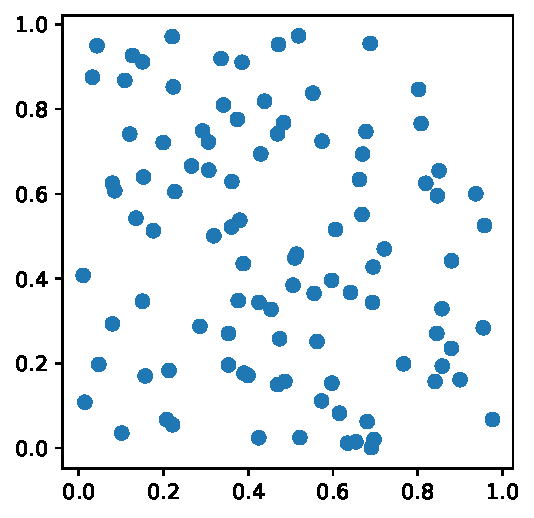
\includegraphics[width=.3\textwidth]{poisson.pdf}\label{subfig:poisson}}
\caption{Examples of the Strauss point process.}
\end{figure}


\begin{qbox}How could you both  quantitatively and qualitatively characterise the different point process you can generate with this function? (Bonus: do it.)
 
\end{qbox}



\begin{pcomment}
\begin{premark}Useful Python function: \pinline{scipy.spatial.distance.pdist}.
\end{premark}
\end{pcomment}


\begin{mcomment}
\begin{mremark}
Useful \matlabregistered{} function: \minline{pdist}.              
\end{mremark}
\end{mcomment}
                


\section{Boolean models analysis (10 points)}
Let us consider a set of binary images of size $1024\times 1024$ made of white particles on a black background. The particles are disks or ellipses of random radius.

\begin{center}
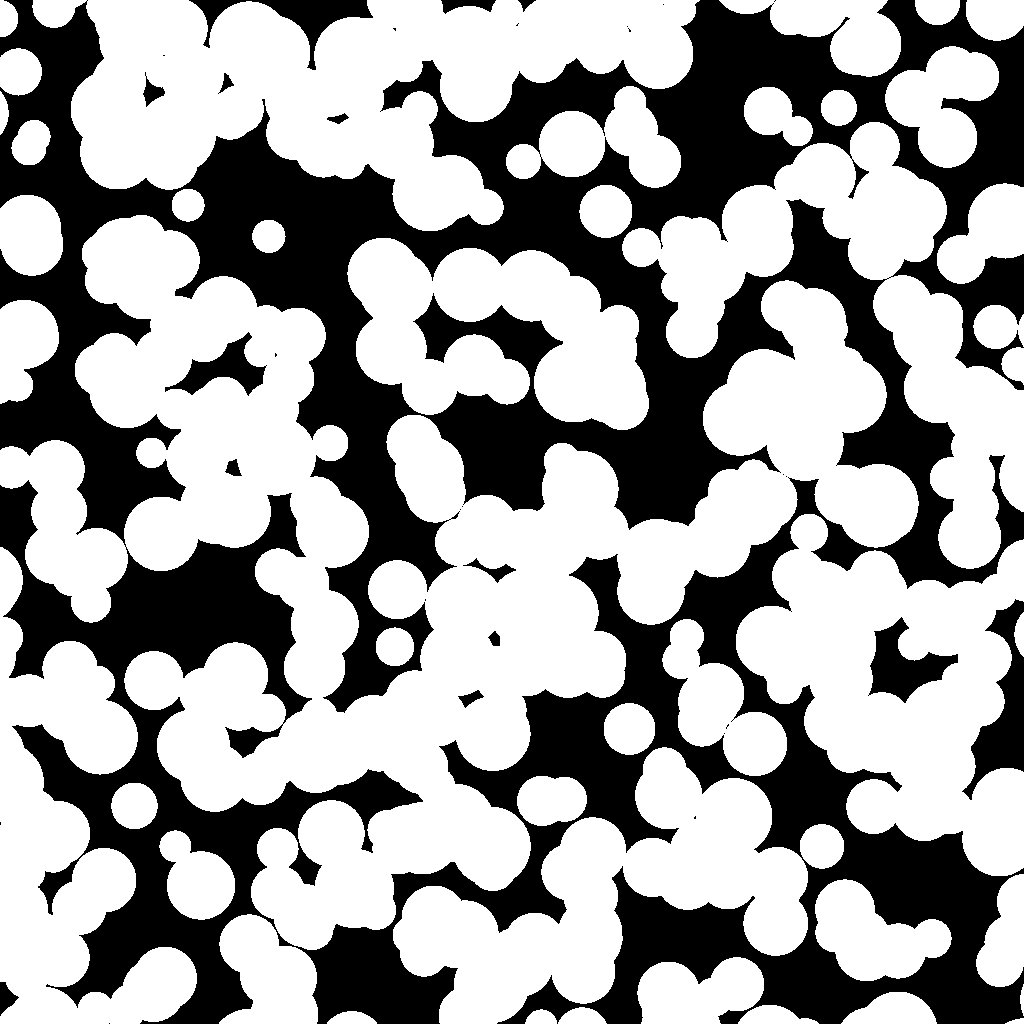
\includegraphics[width=.3\textwidth]{I_400_2.png}
\qquad
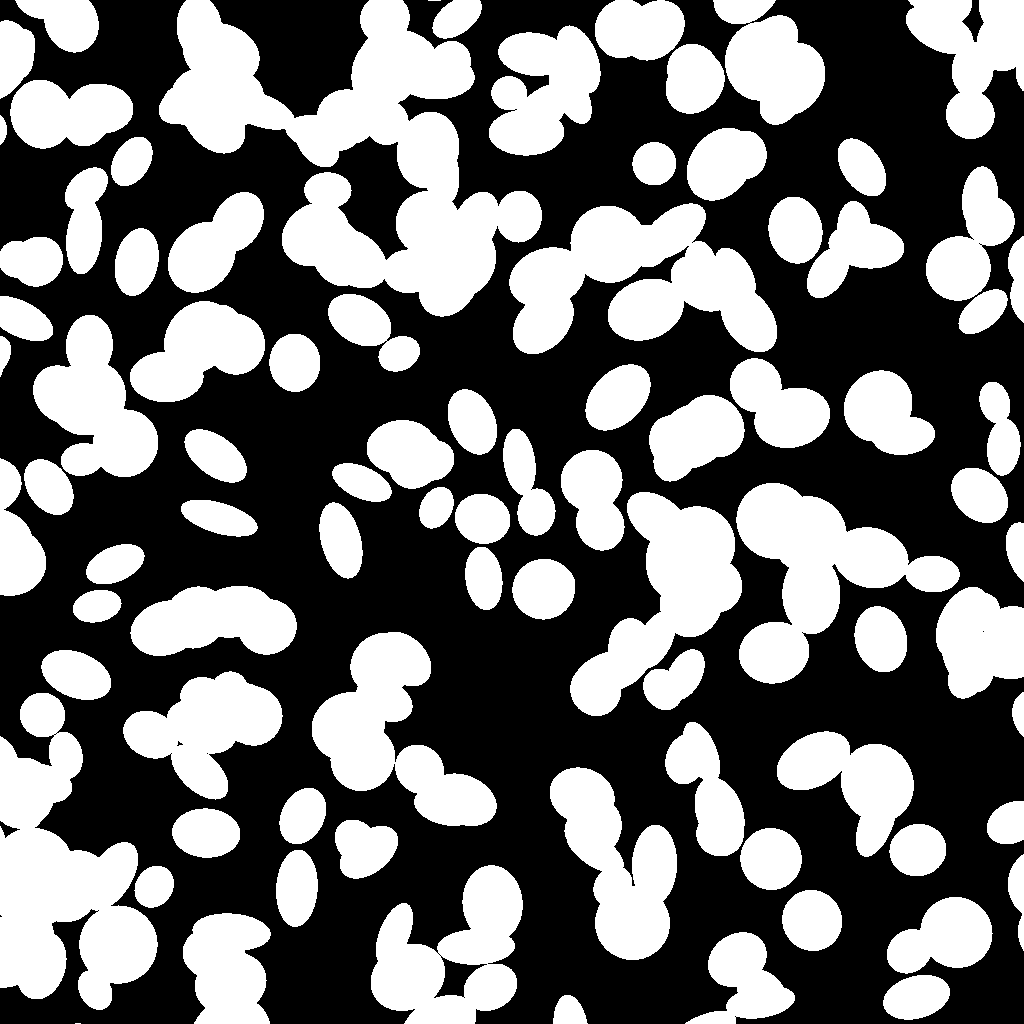
\includegraphics[width=.3\textwidth]{I_250_7.png}
\end{center}

\begin{qbox}
\begin{itemize}\item 
For a disk or an ellipse, what is $x$ (its Euler number)?

\item Propose and implement a method to retrieve the characteristics of the mean particle for each set of images at your disposal: area, perimeter and mean radius for disks; mean equivalent radius for ellipses.
 \item 
Explain your methodology and any assumptions you may have to make.
\end{itemize}

\end{qbox}

We recall the Miles formulas in 2-D:
\begin{align}
\dfrac{A}{W_{size}} & = 1-e^{-\lambda a}\\
\dfrac{P}{W_{size}} & = e^{-\lambda a}\times \lambda p\\
\dfrac{\pi \chi}{W_{size}} & = e^{-\lambda a} \left( \pi\lambda x - \dfrac{1}{4}(\lambda p)^2 \right)
\end{align}

where $A$, $P$ and $\chi$ are the expected value of area, perimeter and euler's number measured on the images, and $a$, $p$ and $x$ their counterpart for the mean particle. The parameter $\lambda$ would be the density of particles and $W_{size}$ the area of the observation window.

\subsection{Useful programming considerations}

\begin{pcomment}
 \begin{premark}
Useful Python functions: \texttt{skimage.measure.area}, \texttt{skimage.measure.perimeter}, \texttt{skimage.measure.euler\_number}.
Optional, yet useful, Python function: \texttt{scipy.optimize.fmin}.
 \end{premark}

 In order to load a set of images contained in a directory, you might use:
 \begin{python}
from glob import glob
import skimage.io

listOfFiles = glob("pix400/*.png")
W = np.zeros((len(listOfFiles), 3))
for i, filename in enumerate(listOfFiles):
    X = skimage.io.imread(filename)
 \end{python}

\end{pcomment}

\begin{mcomment}
 \begin{mremark}
  
Useful \matlabregistered{} functions: \texttt{bwarea}, \texttt{bwperim}, \texttt{bweuler}.
Optional, yet useful, \matlabregistered{} function: \texttt{fminsearch}.
 \end{mremark}

\end{mcomment}




